\documentclass{article} % For LaTeX2e
\usepackage{nips13submit_e,times}
\usepackage{hyperref}
\usepackage{url}
\usepackage{graphicx}
\usepackage{subcaption}
%\documentstyle[nips13submit_09,times,art10]{article} % For LaTeX 2.09


\title{CSC 2515 Project: SVHN}


\author{
Didier Landry\\
Department of Electrical and Computer Engineering\\
University of Toronto\\
\texttt{didier.landry@mail.utoronto.ca} \\
\And
Dustin Kut Moy Cheung\\
Department of Electrical and Computer Engineering\\
University of Toronto\\
\texttt{dustin.kutmoycheung@mail.utoronto.ca} \\
}

% The \author macro works with any number of authors. There are two commands
% used to separate the names and addresses of multiple authors: \And and \AND.
%
% Using \And between authors leaves it to \LaTeX{} to determine where to break
% the lines. Using \AND forces a linebreak at that point. So, if \LaTeX{}
% puts 3 of 4 authors names on the first line, and the last on the second
% line, try using \AND instead of \And before the third author name.

\newcommand{\fix}{\marginpar{FIX}}
\newcommand{\new}{\marginpar{NEW}}

\nipsfinalcopy % Uncomment for camera-ready version

\begin{document}


\maketitle

\begin{abstract}
Detecting and reading text from photographs is a challenging computer vision problem that has garnered a lot of work in recent years. Being able to accurately localize, and recognize arbitrary digits from natural images is hard due to the complex scenes in those images. In this report, we apply convolutional neural networks to learn a unique set of features optimized for this task, and discuss the evolution of our neural network topology to achieve a high accuracy on the validation set. We use over 500,000 labeled digits obtained from the SVHN\cite{svhn} dataset for training. Moreover, we also describe our attempt to localize digits from unconstrained images by using image processing techniques and unsupervised learning.
\end{abstract}

\section{Background}
Convolutional neural networks\cite{lecun_convolutional_svhn} are biologically-inspired neural networks that use identical copies of the same neuron for training, allowing the network to have a large number of units while keeping the number of parameters of those neurons small. The convolutional layers are connected to pooling layers to reduce dimensionality. One popular choice is the max-pooling layer, which extracts the maximum of features over small blocks of the previous layer.

2D convolutional neural networks are used in computer vision to learn features for extraction information. The 2D layer will look at patches of images to generate features such as the detection of the presence of an edge, or a particular texture. Those 2D networks are often stacked together with fully-connected neural networks to form the LeNet family of models, which are extremely popular in computer vision.

Recently, convolutional neural networks have been applied with dropout training\cite{dropout}. Training deep neural networks with a small training set generally leads to overfitting. Dropout is a technique used to prevent overfitting by randomly dropping out units in a neural network. Other popular methods to fix overfitting is to simply stop training when the performance on the validation set starts to get worse, and L2 regularization on the neurons' weights.

All of our training data is provided from the Street View House Numbers(SVHN)\cite{svhn} dataset. It is a popular training set consisting of Street View images cropped to either show single digits (Format 2) and multiple digits (Format 1). Those images are extracted using a combination of automated algorithms and Amazon Mechanical Turk (AMT) framework.


\section{Problem Description}
The project consists of classifying digits from street view images. All the images in the Format 2 dataset have a fixed 32x32 resolution with a digit centered at the image. There are ten classes in total. The images show vast intra-class variations due to image distortions that happen in natural scene pictures. Factors that cause those image distortions include lighting, shadows, motion, and focus blurs.

The Format 1 dataset consists of images with different resolutions with multiple digits in each image. The images are not well cropped and not centered. The task is to first detect the digits with a bounding box, then classify each digit. The images in the Format 1 dataset also show the same image variations as in the Format2 dataset.

To facilitate the process of implementing and debugging the digit recognition, the Format 2 data was used to test the digit recognition neural network. The digit segmentation was treated as a different problem because it (obviously) degrades the quality of the input images fed to the neural network. However, the digit segmentation algorithm produces 32x32 images that could, then, be fed to the neural network for recognition.

\section{Process}
\subsection{Digit Recognition}
\subsubsection{Frameworks Used}
Throughout the project, we use the popular Theano project\cite{theano}, together with Lasagne\cite{lasagne}, numpy, scipy\cite{numpyscipy}, and NoLearn\cite{nolearn} libraries. Most of our experiments are executed using an EC2 machine with a GPU to exploit the speed gains of training with the CUDA framework.

\subsubsection{Basic Neural Network}
Our first approach is to train a basic Neural Network with two hidden layers with the grayscale images of the train dataset. The nonlinearity activation function used for our hidden layers is the Rectifier\cite{relu}, whereas the output layer uses a softmax layer. The grayscale images are normalized before being used as input. The output layer consists of 10 units, each representing a particular digit. The guessed digit from the Neural Network is determined by the unit with the largest value.

\subsubsection{Convolutional Neural Network (CNN)}
We also attempted to add convolutional neural networks to our basic neural network. We added two convolutional and max-pooling layers in between the inputs and the rectifier hidden layers.


\subsubsection{Improvement to CNN}
One of the issues that can be experienced when using deep neural networks is overfitting, where the neural networks overtrain on the training set, while the validation set gets worse. One of the methods to rectify overlearning is by the use of Dropout layers.

Another improvement to our Convolutional Neural Network is to employ pre-processing on our images to boost some features that could help our network train faster and better. One of the most used techniques is the Local Contrast Normalization, which is applied to each of the three color channels of the images.

\subsubsection{Augmenting the training set}
Another way to decrease overfitting in our neural network is to simply augment our training set. To achieve this, we use the extra set (~500k images) available from the SVHN dataset to augment our initial training set of ~ 73k images. We also tried to increase our dataset by adding noise and slightly rotating our existing training set to produce more data.

\subsection{Image Segmentation}
The unsegmented data set contains images of houses' address plates at different levels of zoom of zoom and isolation. Moreover, the number of digits that a given image contains is also unknown. Consequently, separating each individual digit is far from trivial.

One approach could have been to randomly take squares from the image and train a classifier to decide whether it contains a digit or not. This could have worked rather well if the goal was just to find digits in an image. However, for segmentation (one image per digit, centered), its performance would have been random at best. Since, to properly decode an address, the information contained in the number of digits and their order is as important as the digits themselves, this approach was rejected.

Accordingly, here, we wrote an algorithm loosely inspired on the MATLAB OCR example\cite{automaticdetect}.

First, the images are preprocessed: they are resized to a height of 200 pixels while keeping the aspect ratio the same and converted to grayscale.

\begin{figure}[!htb]
\minipage{0.32\textwidth}
  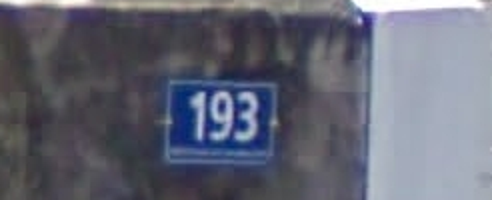
\includegraphics[width=\linewidth]{images/image02}
  \caption{Original Image (2200.png in training set)}
  \label{fig:orig}
\endminipage\hfill
\minipage{0.32\textwidth}
  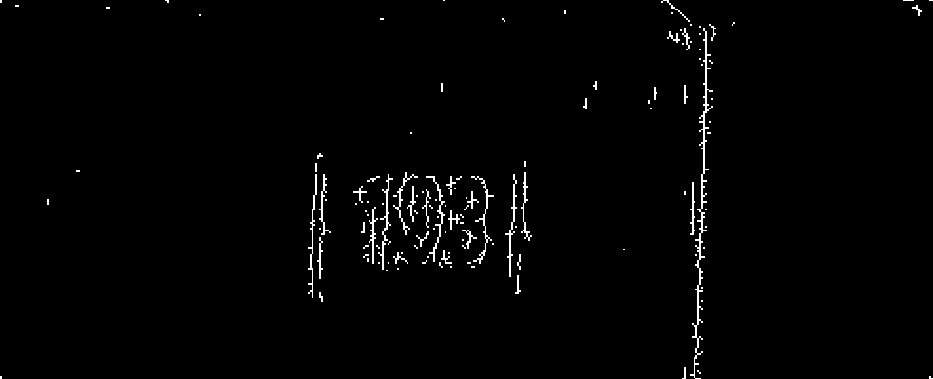
\includegraphics[width=\linewidth]{images/image06}
  \caption{Vertical Edges (Sobel vert. edge detection)}
  \label{fig:vertical}
\endminipage\hfill
\minipage{0.32\textwidth}%
  
\includegraphics[width=\linewidth]{images/image00}
  \caption{Mask obtained by morphological closing, after filtering}
  \label{fig:mask}
\endminipage
\end{figure}

The second step is to find the areas of the image that have a high probability of containing text (an approach similar to that of A. Coates et. al.'s "detection"\cite{coates2011text}). For that, we apply a sobel vertical edge detection algorithm and, then, morphological closing on the found edges (very scattered) to create connected regions. This worked well because the vertical boundaries in numbers tend to create a rectangular blob of points that, when morphologically closed, completely contains the digit (Figure~\ref{fig:vertical} \& ~\ref{fig:mask}). Vertical edges such as the wall, in this example, get filtered easily because, after closing, they create really narrow regions.

Depending on the image, this preliminary analysis can produce a lot of possibilities. To solve this problem, the candidate connected zones are filtered by size, aspect ratio and solidity. Areas that are too narrow, fat or have a low solidity (level of vertical gradients in a box containing the connected zone) are discarded. The zone that has the greatest probability of containing a digit is then passed to the next step.

\begin{figure}[!htb]
\minipage{0.45\textwidth}
  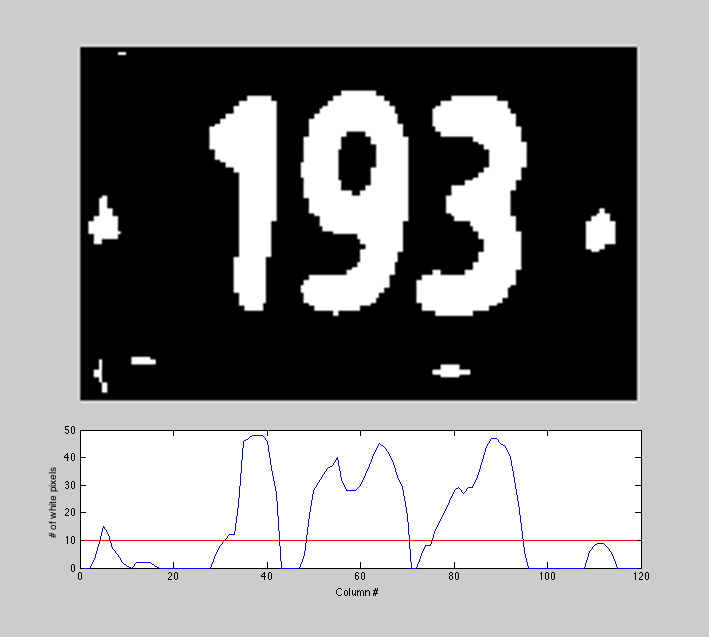
\includegraphics[width=\linewidth]{images/image08}
  \caption{Digit splitting based on # of white pixels per column. The red line is the threshold.}
  \label{fig:thres}
\endminipage\hfill
\minipage{0.45\textwidth}
  
\includegraphics[width=\linewidth]{images/image04}
  \caption{Split Zones. Leftmost zone was discarded because of its small width}
  \label{fig:split}
\endminipage\hfill
\end{figure}

The third step is to detect the number of digits present in the previously found area. For that, the image is turned into binary (black and white) using Otsu’s thresholding method\cite{otsu1975threshold,graythresh} . Then, after inverting the image if the background is white, the number of white pixels in each column (assumed to be the digit) is counted. If it falls below a threshold (that is a function of the maximum number of white pixels in the image’s column), a split point is saved (see Figure~\ref{fig:thres} \& ~\ref{fig:split}).


\begin{figure}
\begin{subfigure}{.3\textwidth}
  \centering
  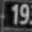
\includegraphics[width=.8\linewidth]{images/image03}
\end{subfigure}%
\begin{subfigure}{.3\textwidth}
  \centering
  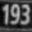
\includegraphics[width=.8\linewidth]{images/image07}
\end{subfigure}
\begin{subfigure}{.3\textwidth}
  \centering
  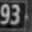
\includegraphics[width=.8\linewidth]{images/image01}
\end{subfigure}
\caption{Final Output}
\label{fig:output}
\end{figure}

Finally, the split zones are, again, filtered by width and cropped into 32x32 pixels images (extending laterally to get a 1:1 aspect ratio, if necessary) (Figure~\ref{fig:split} \& ~\ref{fig:output}).


\section{Experimental Results}
\subsection{Digit Recognition}

\begin{center}
\begin{table}[h]
  \begin{tabular}{ | p{10cm} || c ||}
    \hline
    Algorithm & Validation Accuracy \% \\ \hline \hline
    NN with Regular Hidden layers (1 hidden layer, 300 units
trained on complete training set) & 79.43 \\ \hline
NN with Convolutional Layers
(2 convolutional layers, 24 and 32 filters and max-pooling
1 hidden layer, 300 units
trained on complete training set) & 89.37 \\ \hline
NN with Convolutional Layers and Contrast Normalization
(2 convolutional layers, 24 and 32 filters and max-pooling
1 hidden layer, 300 units
trained on complete training set) & 90.15 \\ \hline
NN with Convolutional Layers and Contrast Normalization and Dropout
(2 convolutional layers, 24 and 32 filters and max-pooling
1 hidden layer, 300 units, dropout layer
trained on complete training set) & 90.89 \\ \hline
  \end{tabular}

\caption{Algorithm and Accuracy}
\label{table:algo}
\end{table}
\end{center}

As shown in Table~\ref{table:algo}, the greatest accuracy jump came from using convolutional layers in the neural network. Indeed, accuracy jumped by almost 10\%, which was an even more dramatic effect than adding ~500k extra training examples (~6\% improvement).

This is not a surprising result since convolutional layers are known to be good at image processing. The layers typically learn features such as contrast and edges. Strangely, however, adding a third or fourth convolutional layer degraded the results. This might be because, given the size of the images, adding extra layers was superfluous.

On the other hand, adding contrast normalization had very little effect on the accuracy. It’s possible that the lack of contrast in the original image was just compensated by some weights being higher (more “sensitive” contrast thresholds). When processing the images with improved contrast, the network would just have learned to be less sensitive while learning the same features. This makes sense; increasing contrast only “boosts” information already present in the image at the first place\cite{lenet5}.


\begin{center}
	\begin{table}[!h]
		  \begin{tabular}{ | l || c ||}
		    \hline
		    \# of training examples & Accuracy \% \\ \hline \hline
		    73,257 (just the training set) & 89.28 \\ \hline
		    100,000 & 93.74 \\ \hline
		    200,000 & 95.06 \\ \hline
		    300,000 & 95.69 \\ \hline
		    400,000 & 96.00 \\ \hline
		    500,000 & 96.13 \\ \hline
		    604,388 (all of training + all of extras) & 96.50 \\ \hline
		  \end{tabular}
	  \caption{Accuracy vs Training Examples}
	  \label{table:train}
	\end{table}
\end{center}

\begin{center}
\begin{figure}[!htb]
  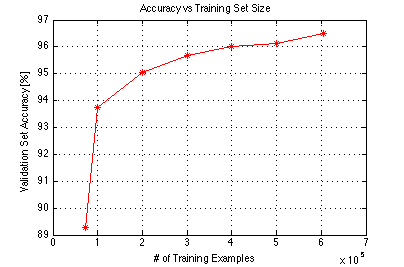
\includegraphics[width=0.8\linewidth]{images/image05}
  \caption{Accuracy vs. Training Examples. (2 convolutional layers, 24 and 32 filters and max-pooling 1 hidden layer, 300 units)}
  \label{fig:accuracy}
\end{figure}
\end{center}


The next thing that greatly improved the results was to augment the training set with some examples taken from the “extras” set. This confirms the general intuition that “more data is better”.  Figure~\ref{fig:accuracy} and Table~\ref{table:train} show the accuracies obtained with different numbers of training examples after 10 epochs.

\subsection{Image Segmentation}

It is important to point out that the digit segmentation algorithm is mostly an engineered solution (in that it doesn’t learn from the data); it just applies decisions based on hard-coded thresholds, gradients and masking.

This is because this engineered solution systematically performed better than the machine learning techniques we used and that any attempt to integrate machine learning algorithms degraded the results. Below are a few of the techniques that were tried but later abandoned.

\subsubsection{Better Boundaries}
An attempt to use a more advanced edge detection algorithm, P. Isola et. al.’s crisp boundary detection\cite{isola2014crisp}, was made without success. Indeed, with low contrast pictures, it would detect tiles due to colour imperfections in the image file’s encoding while, in images where a strong colour contrast that is not due to the address’ digits is present (such as the edge of a wall), it would completely disregard the lower contrast changes due to the digits.

\subsubsection{PCA for Segmentation}
In order to make the separation of the digits easier, an attempt was made to use PCA to generate the histogram in Fig. 4 (and to rectify the image when the address was diagonal). This, for instance, would have made it easier to separate numbers that are placed in diagonal because it would have been rotated to an horizontal orientation (the current algorithm tends to fail at this task because of the vertical overlap between the numbers). However, this approach was abandoned because it also had major adverse effects, such as a tendency to flip the image vertically or horizontally that made it perform worse than a simple count of white pixels.

\subsubsection{kNN for Segmentation}
Further, kNN was tried as a way to locate the centers of the digits. The white pixel count was be used to guess a value for k and, then, the image was split using the centroids found by kNN on the thresholded image. This caused more errors than a simple split however, because, even if the number of digits found was correct, the centroids were sometimes distributed vertically (i.e. two centroids on the same number) instead of all horizontally. Forcing the kNN to be only horizontal produced slightly better results but was still not as good as a simple split because it was sensitive to noise (address plate edges) and weight distributions in the digits (a “5” typically has a centroid in its upper-left portion, for instance).

\subsubsection{Results}
The segmentation results are reported in Table~\ref{table:segmentation}. Please note that the accuracy is based on a “success” being defined as properly isolating and centering ALL the digits in an image (not more or less). For instance, the case where all the digits of an address were found properly where but the edge of the number plate was mistaken for an “1” would be considered a “fail”. 

Also, since this definition of success is too variable for a computer to properly evaluate it, the “successes” had to be counted manually. This, unfortunately, introduces a bias in the numbers below as it limits the number of examples that can be used to compile the accuracy statistics.

\begin{center}
	\begin{table}[h]
  		\begin{tabular}{ | l || c ||}
	    	\hline
		    Examples (treated with this algorithm) & Accuracy (hand-counted) \% \\ \hline \hline
		    100 examples from training set (2200 to 2300.png) &  36 \\ \hline
		    100 examples from extras set (3000 to 3100.png) & 37 \\
		    \hline
        \end{tabular}
		  \caption{Examples vs Accuracy for Image Segmentation}
		  \label{table:segmentation}
  	\end{table}
\end{center}

\section{Discussion and Conclusion}
\subsection{Scaling with Millions of Examples}
Scaling our current convolutional neural network to millions of examples is incredibly challenging. Luckily, in Lasagne, a lot of optimizations happen in the background. For instance, the batch size is selected automatically depending on the number of examples.

Even though Lasagne and Theano ultimately produces CUDA code that can be run on a GPU, there are further optimizations that could be achieved by using a pure CUDA approach and getting rid of Python dependencies along the way. 

One way to scale our training is to simply use a distributed neural network spanning across several machines. With this amount of data, the overhead involved with communication between the different machines become negligible compared to the speed gain in training in parallel. An example of such a distributed network is DistBelief\cite{dean2012large}, developed at Google.

Another way is to simply decrease the pixels of each image used to a smaller size. By having less pixels to train on, the training speed will increase, albeit at the expense of losing some information.

\subsection{Digit Recognition}
The input representation of the images into the Convolutional Neural Network consists of grayscale images obtained from the original RGB images. In future work, this could further be improved by using the YUV representation of those images. YUV representations tend to be less sensitive to different lighting conditions and may help reduce the intra-class variations in the SVHN dataset.

The number of layers in our convolutional neural network are relatively small compared to what some of the current solutions are using. It will be interesting to see how our results are affected by deeper networks, more filters in our convolutional layer and even more training data. 

Alternate pooling layers could also be explored. Some research points to the use of Lp-Pooling\cite{lecun_convolutional_svhn} as a superior pooling layer to the max-pooling we are currently using.

We could also explore the use of Maxout Networks\cite{maxout} with our current network to see if it helps with delaying overfitting.

\subsection{Image Segmentation}
The image segmentation algorithm could be improved to allow for more than one zone of high probability to contain a digit. Currently, if the numbers of the address are too far apart in the image, they get “boxed” separately and, in the end, only one number gets isolated properly. This is because, after the morphological closing of the vertical gradients, all the numbers are assumed to be in the same connected zone (this was a simplifying assumption that proved to be correct in most cases).

It would also be interesting to continue to investigate to find machine learning techniques that could exploit some information that comes with the Format 1 images; the boxes. Indeed, each image comes with the location and size of boxes that surround the each digit. Perhaps, using the number of boxes, a classifier could be trained in a supervised manner to find the number of digits in each image. 

\bibliographystyle{plain}
\bibliography{ml}
\end{document}
